\subsection{From Multi-Process to Multi-Enclave}
\label{sec:multiproc}

Upon existing platforms using \sgx{}, there is no
multi-process abstractions of any kinds that has been supported so far,
either in \haven{} or other systems.
The main challenge against
implementing multi-process abstractions in enclaves
is to share enclave pages,
for either Linux-style copy-on-write {\tt fork}'ing or
sharing abstraction states.
Fortunately, \graphene{} implements multi-process support
including {\tt fork}, {\tt execve}, signals, System V IPC, etc,
without any need to share pages.
The {\it zero-sharing} nature of \graphene{} makes it possible
to support multi-process abstractions in enclaves
without any architecture changes.

In this section we will describe how \sysname{} securely creates
processes in new enclaves,
for supporting {\tt fork} and {\tt execve},
and implements inter-process communication
(namespace coordination, signals, System V IPC, etc)
with process isolation.

\subsection{Forking into New Enclaves}
\label{sec:multiproc:fork}

\begin{figure}[t!]
\centering
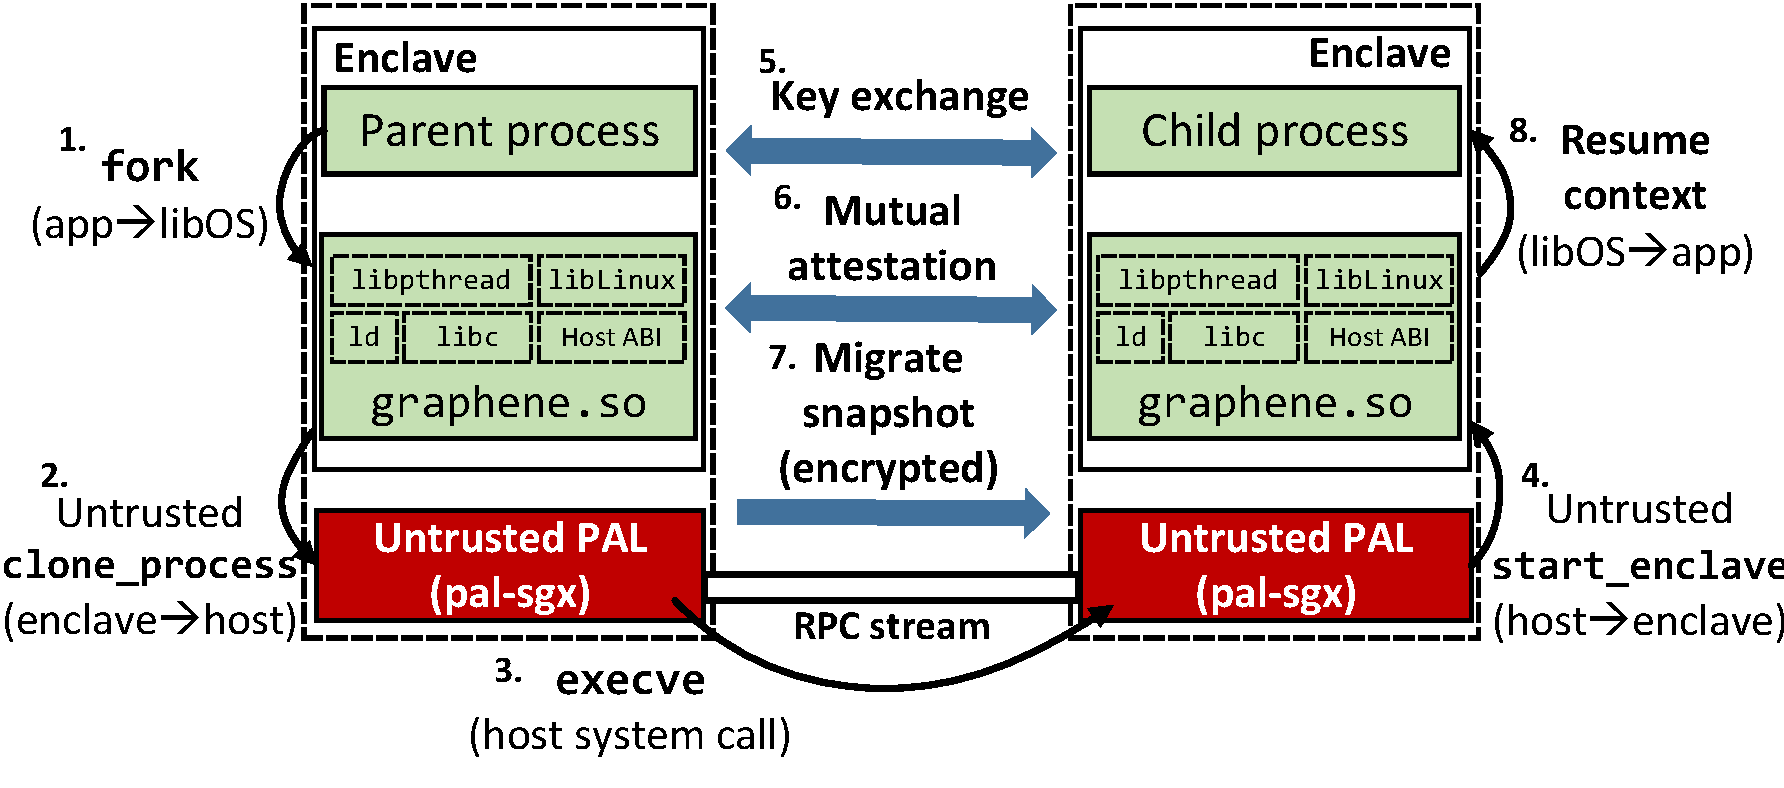
\includegraphics[width=5in]{graphene-sgx/figures/fork.pdf}
\footnotesize
\caption[Process creation in \sysname{}]
{Process creation in \sysname{}.
Numbers show the order of operations.
When a process forks, \sysname{} calls {\tt execve} system call
on the untrusted host,
to create a clean enclave with the same \libos{} image.
Then the two enclaves build up the mutual trust by
exchanging a session key, verifying attestation of each other,
and migrating the process snapshot from the parent.}
\label{fig:fork}
\end{figure}

To secure process creation across enclaves,
\sysname{} is capable of building up the trust to newly launched enclaves,
through cooperation with an untrusted host.
Once a clean and trusted new enclave is launched,
The parent process will send a snapshot to the new one,
to create a clone of itself.
Snapshotting and migrating process states
is a feature robustly implemented and heavily used in \graphene{} \libos{},
of which we simply inherit the design.

When a process in \sysname{} forks,
because the parent and the child will be running the same binary,
both enclaves can simply be expected to have the same measurement.
To build up the trust, the two processes will open an encrypted channel
using a session key,
and exchange attestation generated by the processor.
Once both sides have confirmed the integrity of the other,
the parent process is safe to send its snapshot, encrypted, to the child
through the said channel.
The child process will restore the snapshot in its own enclave,
making it a clone of its parent.
The design of process creation in \sysname{} is shown as Figure~\ref{fig:fork}.

Forking in \sysname{} mainly defends against 3 types of attacks
from the untrusted host:

\begin{compactenum}

\item The host pretends to be the child enclave, to expose the process snapshot
sent from the parent.

\item The host pretends to be the parent enclave, to compromise the
child process using a malicious process snapshot.

\item The untrusted host becomes a man-in-the-middle, which bounces
encrypted messages between the child and parent enclaves, with session keys
negotiated with both sides.

\end{compactenum}

As described earlier, attacks 1 and 2 are prevented by mutual attestation
between the parent and the child,
and encrypting the channel for sending the snapshot.
The attestation signed by the processor proves that both entities communicating
are valid \sysname{} enclaves,
and encrypting the channel prevents the snapshot being eavesdropped or
counterfeited by the host.

To defend against attack 3 (the man-in-the-middle attack), we take advantage of
a user-customized 512-bit field
in the attestation structure generated and signed by \sgx{}.
This field is filled with a SHA-256 hash value of the agreed session key,
and the current enclave ID,
to prove that the attested enclave is the one who agrees on the key.

Once a parent enclave forks a child, by default the child must be trusted
to maintain its own security,
because the migrated snapshot discloses all information in the parent.
Unless the binary run in the parent enclave ensures
that no secrets is stored in the enclave memory at the time of snapshotting,
the parent enclave cannot simply drop the trust against the child.
For example, a pre-forked Apache web server may want to keep each worker
that responds to HTTP requests isolated,
to avoid being compromised by one attacked worker.
\graphene{} \libos{} provides an API for applications like Apache to explicitly
specify isolation to untrusted child processes.
\sysname{} inherits the ability of dynamic process isolation,
but developers are responsible for keeping confidential information
from the untrusted children.

\paragraph{Implementing {\tt execve}.}
Unlike {\tt fork}, {\tt execve} is used to
start processes with specified binaries, often different from the callers'.
When a thread in the process, either single-threaded or multi-threaded,
calls {\tt execve} in \sysname{},
\libos{} will migrate the calling thread to a new process,
with clean process states except opened files cloned from the parent.

The main challenge for implementing {\tt execve} is to
identify trusted binaries that can be loaded into new enclaves as child processes.
Consider the case where the parent process and its child shares
a multi-process abstraction (e.g., message queue).
Even if only the parent side is provisioned by the client, the child side
can still potentially compromise the secrets,
by exploiting vulnerabilities in the shared abstraction.
The trust between the parent and the child must be mutual,
unless the two enclaves are strictly isolated.

To identify binaries that can be trusted (either as parents or children)
during process creation,
\sysname{} requires each binary ported for an application,
to be shipped with a list of binaries that can be {\tt execve}'d,
and those that can be callers of {\tt execve} to the said binary.
Each binary in the list is identified by its measurement, which is mutually attested
between the parent and the child during process creation.
This list must be signed by a private key provided by the client,
while the public key must be included in the enclave measurement of the binary.

\subsection{Securing Inter-Process Coordination}
\label{sec:multiproc:ipc}

After process creation, a multi-process application often cooperate
through shared abstractions between processes,
such as signals or message queues.
For \libos{}, OS states for these shared abstractions must be shared
though inter-process coordination, for mainly two purposes.
First, for each abstraction, \libos{} needs to maintain the state
in one of its instances.
Second, \libos{} must maintain the namespace states to identify and locate the
abstraction states.

\graphene{} implements a wide range of multi-process abstractions and namespaces,
by passing messages over RPC streams among processes.
Such a design is perfect for porting multi-process applications to enclaves.
The benefit of sharing abstraction by RPC coordination are that
the enclaves will not have to share any memory to
coordinate abstraction states,
and the RPC streams can be secured by the enclaves instead of the host.

In \graphene{}, security isolation among multi-process abstractions,
regardless of their semantics,
are enforced by isolating the RPC streams used for coordination.
Unfortunately, \sysname{} cannot trust the host to faithfully isolate
the RPC streams.
Each enclave launched for an application must secure inter-process coordination
spontaneously, by only communicating to enclaves that it has attested
and exchanged secret keys with.
Because inter-process coordination is completely transparent
to the applications,
all information sent over RPC streams must be encrypted,
because \libos{} cannot determine whether the information may contain any secret.





